% Options for packages loaded elsewhere
\PassOptionsToPackage{unicode}{hyperref}
\PassOptionsToPackage{hyphens}{url}
\documentclass[
  ignorenonframetext,
]{beamer}
\newif\ifbibliography
\usepackage{pgfpages}
\setbeamertemplate{caption}[numbered]
\setbeamertemplate{caption label separator}{: }
\setbeamercolor{caption name}{fg=normal text.fg}
\beamertemplatenavigationsymbolsempty
% remove section numbering
\setbeamertemplate{part page}{
  \centering
  \begin{beamercolorbox}[sep=16pt,center]{part title}
    \usebeamerfont{part title}\insertpart\par
  \end{beamercolorbox}
}
\setbeamertemplate{section page}{
  \centering
  \begin{beamercolorbox}[sep=12pt,center]{section title}
    \usebeamerfont{section title}\insertsection\par
  \end{beamercolorbox}
}
\setbeamertemplate{subsection page}{
  \centering
  \begin{beamercolorbox}[sep=8pt,center]{subsection title}
    \usebeamerfont{subsection title}\insertsubsection\par
  \end{beamercolorbox}
}
% Prevent slide breaks in the middle of a paragraph
\widowpenalties 1 10000
\raggedbottom
\AtBeginPart{
  \frame{\partpage}
}
\AtBeginSection{
  \ifbibliography
  \else
    \frame{\sectionpage}
  \fi
}
\AtBeginSubsection{
  \frame{\subsectionpage}
}
\usepackage{iftex}
\ifPDFTeX
  \usepackage[T1]{fontenc}
  \usepackage[utf8]{inputenc}
  \usepackage{textcomp} % provide euro and other symbols
\else % if luatex or xetex
  \usepackage{unicode-math} % this also loads fontspec
  \defaultfontfeatures{Scale=MatchLowercase}
  \defaultfontfeatures[\rmfamily]{Ligatures=TeX,Scale=1}
\fi
\usepackage{lmodern}
\ifPDFTeX\else
  % xetex/luatex font selection
\fi
% Use upquote if available, for straight quotes in verbatim environments
\IfFileExists{upquote.sty}{\usepackage{upquote}}{}
\IfFileExists{microtype.sty}{% use microtype if available
  \usepackage[]{microtype}
  \UseMicrotypeSet[protrusion]{basicmath} % disable protrusion for tt fonts
}{}
\makeatletter
\@ifundefined{KOMAClassName}{% if non-KOMA class
  \IfFileExists{parskip.sty}{%
    \usepackage{parskip}
  }{% else
    \setlength{\parindent}{0pt}
    \setlength{\parskip}{6pt plus 2pt minus 1pt}}
}{% if KOMA class
  \KOMAoptions{parskip=half}}
\makeatother
\usepackage{longtable,booktabs,array}
\newcounter{none} % for unnumbered tables
\usepackage{calc} % for calculating minipage widths
\usepackage{caption}
% Make caption package work with longtable
\makeatletter
\def\fnum@table{\tablename~\thetable}
\makeatother
\usepackage{graphicx}
\makeatletter
\newsavebox\pandoc@box
\newcommand*\pandocbounded[1]{% scales image to fit in text height/width
  \sbox\pandoc@box{#1}%
  \Gscale@div\@tempa{\textheight}{\dimexpr\ht\pandoc@box+\dp\pandoc@box\relax}%
  \Gscale@div\@tempb{\linewidth}{\wd\pandoc@box}%
  \ifdim\@tempb\p@<\@tempa\p@\let\@tempa\@tempb\fi% select the smaller of both
  \ifdim\@tempa\p@<\p@\scalebox{\@tempa}{\usebox\pandoc@box}%
  \else\usebox{\pandoc@box}%
  \fi%
}
% Set default figure placement to htbp
\def\fps@figure{htbp}
\makeatother
\setlength{\emergencystretch}{3em} % prevent overfull lines
\providecommand{\tightlist}{%
  \setlength{\itemsep}{0pt}\setlength{\parskip}{0pt}}
% Auto-generated by infrastructure/rendering/_pdf_latex_helpers.py::extract_math_font_preamble.
% Minimal header passed to Pandoc via -H so Beamer slides pick up the same math font
% as the combined-PDF path. Adjust the manuscript's preamble.md to change the font globally.
\usepackage{unicode-math}
\setmathfont{latinmodern-math.otf}
\usepackage{bookmark}
\IfFileExists{xurl.sty}{\usepackage{xurl}}{} % add URL line breaks if available
\urlstyle{same}
\hypersetup{
  hidelinks,
  pdfcreator={LaTeX via pandoc}}

\author{\texorpdfstring{}{}}
\date{}

\begin{document}

\section{Appendix A: Syntactic and Semantic Case Assignment
Diagrams}\label{sec:syntactic-diagrams}

\begin{frame}[allowframebreaks]{Appendix A: Syntactic and Semantic Case
Assignment Diagrams}
This appendix presents a curated panel of syntactic constituency-style
diagrams paired with their categorical pregroup type derivations,
covering eight linguistically significant case assignment
constructions---from simple intransitive clauses to complex embedded
relative clauses with ditransitive verbs. The figure synthesizes the
formal correspondences developed throughout the manuscript, making
explicit how each surface syntactic pattern maps to a specific morphism
composition in the pregroup grammar.
\end{frame}

\begin{frame}[fragile,allowframebreaks]{Syntactic Trees and Pregroup
Types: Eight Constructions}
\protect\phantomsection\label{syntactic-trees-and-pregroup-types-eight-constructions}
The figure below (\autoref{fig:syntactic-panel}) presents eight
constructions arrayed in two rows of four panels, each panel containing:

\begin{enumerate}
\tightlist
\item
  \textbf{Syntactic tree} (top): a constituency-style diagram with arcs
  linking argument to predicate, nodes colour-coded by case role
  following the palette of
  \href{11b_notation.md\#sec:notation-linguistic}{Linguistic Terms}.
\item
  \textbf{Pregroup type formula} (bottom): the formal typing derivation
  from \autoref{sec:case-type-logic}, showing how Cup contractions
  collapse all argument wires to sentence type \(s\).
\end{enumerate}

The constructions in \autoref{tbl:appendix-syntactic-constructions} span
a deliberate difficulty gradient:

\begin{longtable}[]{@{}
  >{\centering\arraybackslash}p{(\linewidth - 6\tabcolsep) * \real{0.1316}}
  >{\raggedright\arraybackslash}p{(\linewidth - 6\tabcolsep) * \real{0.3158}}
  >{\centering\arraybackslash}p{(\linewidth - 6\tabcolsep) * \real{0.1316}}
  >{\centering\arraybackslash}p{(\linewidth - 6\tabcolsep) * \real{0.4211}}@{}}
\caption{Appendix A panel index: eight constructions and their
categorical complexity
indicators.}\label{tbl:appendix-syntactic-constructions}\tabularnewline
\toprule\noalign{}
\begin{minipage}[b]{\linewidth}\centering
Panel
\end{minipage} & \begin{minipage}[b]{\linewidth}\raggedright
Construction
\end{minipage} & \begin{minipage}[b]{\linewidth}\centering
Roles
\end{minipage} & \begin{minipage}[b]{\linewidth}\centering
Type Complexity
\end{minipage} \\
\midrule\noalign{}
\endfirsthead
\toprule\noalign{}
\begin{minipage}[b]{\linewidth}\centering
Panel
\end{minipage} & \begin{minipage}[b]{\linewidth}\raggedright
Construction
\end{minipage} & \begin{minipage}[b]{\linewidth}\centering
Roles
\end{minipage} & \begin{minipage}[b]{\linewidth}\centering
Type Complexity
\end{minipage} \\
\midrule\noalign{}
\endhead
1 & Intransitive (NOM) & NOM, V & 2 boxes, 1 Cup \\
2 & Transitive (NOM+ACC) & NOM, V, ACC & 3 boxes, 2 Cups \\
3 & Ditransitive (NOM+DAT+ACC) & NOM, V, DAT, ACC & 4 boxes, 3 Cups \\
4 & Passive voice (Patient→NOM) & NOM, V, INS & 3 boxes +
\(\sigma{}\) \\
5 & Ergative clause (ERG+ABS) & ERG×2, ABS×2, V & 5 boxes, 2 Cups \\
6 & Benefactive (NOM+DAT+ACC+oblique) & NOM, V, ACC, DAT & 4 boxes, 3
Cups \\
7 & Relative clause (embedded NOM) & NOM×2, V1, V2 & 6 boxes, 3 Cups \\
8 & Causative + Adj + Adv (complex) & NOM, V, ACC, V2, ADV & 12 boxes, 5
Cups \\
\bottomrule\noalign{}
\end{longtable}

The monotonic increase in Cup count and box count across rows is
precisely what \autoref{eq:eq-4-4} captures as the categorical
complexity \(\kappa{(D)}\): each additional argument slot requires one
additional Cup contraction, and each modifier requires one additional
Box--Cup pair.

\begin{block}{Ergative Clauses and the Alignment Functor}
\protect\phantomsection\label{ergative-clauses-and-the-alignment-functor}
Panel 5 (Ergative clause) uses the Warlpiri example from
\autoref{sec:case-systems}: \emph{Mariyk-angku} (ERG) \emph{yapaku
wawirri} (ABS) \emph{parnta-nu} (chased). The pregroup typing is
structurally identical to the transitive (Panel 2), but the
morphological realisation is governed by the alignment functor
\(F_{\mathrm{ERG}}: \mathcal{U} \to \mathcal{L}_{\mathrm{Warlpiri}}\)
from \autoref{sec:case-systems}, which maps \(A \mapsto \mathrm{ERG}\)
and \(S = P \mapsto \mathrm{ABS}\) rather than
\(A = S \mapsto \mathrm{NOM}\).
\end{block}

\begin{block}{Passivisation as a Swap Morphism}
\protect\phantomsection\label{passivisation-as-a-swap-morphism}
Panel 4 illustrates passivisation: in \emph{Bob is chased by Alice}, the
patient Bob is promoted to subject position (NOM) while Alice is demoted
to an oblique instrumental (INS). Formally, this is the Swap morphism
\(\sigma_{A,B}: A \otimes B \to B \otimes A\) introduced in
\autoref{sec:case-type-logic}. The pregroup typing includes a
\(\sigma{}\) marker indicating that the type permutation is not a simple
contraction sequence but requires an explicit braiding operation.
\end{block}

\begin{block}{Relative Clauses and Wire Threading}
\protect\phantomsection\label{relative-clauses-and-wire-threading}
Panel 7 (Relative clause) is the most structurally novel: in \emph{The
man the dog chased ran}, the head noun \emph{man} is simultaneously the
subject of \emph{ran} and the implicit object of \emph{chased} (the gap
site). The pregroup type formula
\(n \cdot n^l \cdot n \cdot (n^r \cdot n \cdot n^l) \cdot (n^r \cdot s) \Rightarrow s\)
shows how the relative-clause verb type \(n^r \cdot n \cdot n^l\)
threads the shared entity wire through two predicate slots --- exactly
the entity persistence mechanism that DisCoCirc's state wires formalise
at discourse level (\autoref{sec:discocirc-discourse}).
\end{block}

\begin{block}{Complex Construction and the Complexity Metric}
\protect\phantomsection\label{complex-construction-and-the-complexity-metric}
Panel 8 (Causative + Adj + Adv) reaches the highest complexity: 12 boxes
and 5 Cup contractions. This corresponds to a categorical complexity
value of \(\kappa = 12 + 5 = 17\), placing it at the upper end of the
single-sentence range plotted in \autoref{fig:complexity-comparison}.
The formula illustrates how clausal complement embedding (the causative
taking a VP complement) adds a full additional layer of type nesting
beyond even the ditransitive.

\begin{figure}
\centering
\pandocbounded{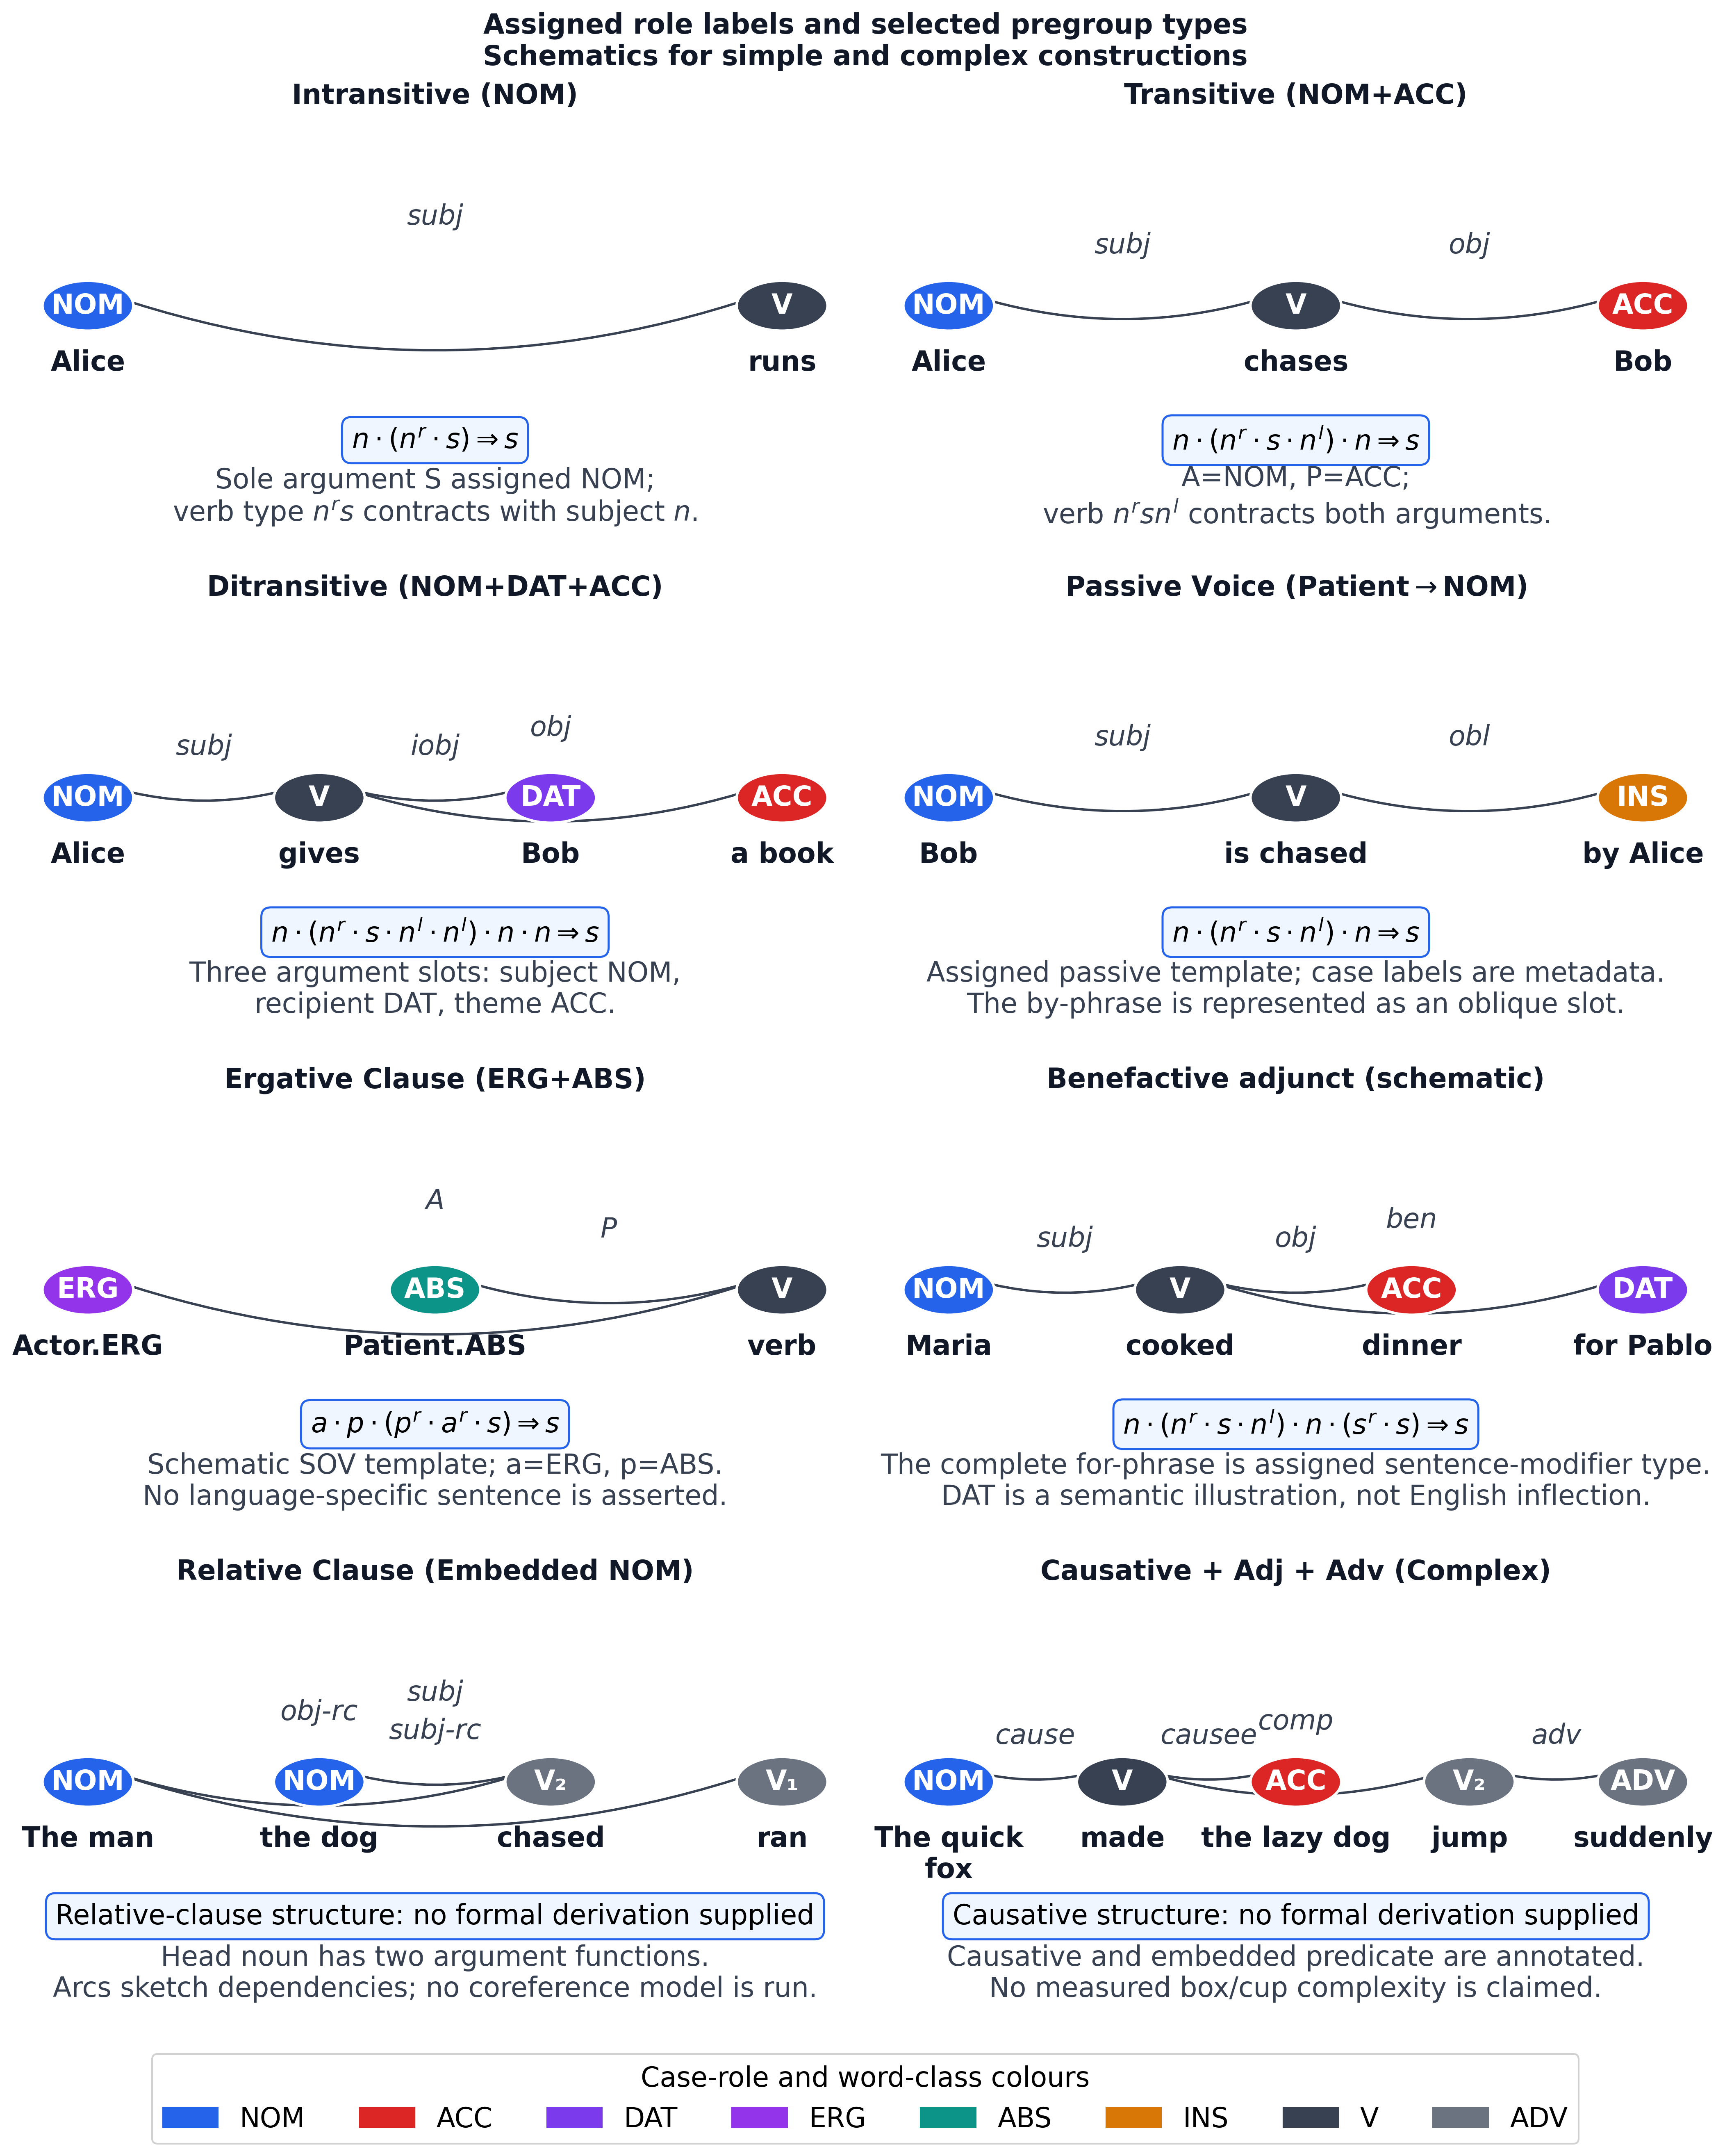
\includegraphics[keepaspectratio,alt={Compositional complexity increases monotonically from intransitive to causative constructions across eight case-assignment patterns. Multi-panel diagram ordered by categorical complexity \textbackslash kappa(D) (). Top of each panel: constituency-style syntactic tree with argument arcs and colour-coded case roles (Blue=NOM, Red=ACC, Violet=DAT, Purple=ERG, Teal=ABS, Dark=V). Bottom of each panel: categorical pregroup type formula showing Cup contractions that collapse argument wires to sentence type s. Panels 1--4 cover nominative-accusative (intransitive, transitive, ditransitive, passive); Panels 5--6 show ergative-absolutive and benefactive; Panels 7--8 demonstrate relative-clause embedding and causative complex predicates. Cup count and box count increase monotonically across panels, directly instantiating \textbackslash kappa(D). Generated programmatically from src.visualization.syntactic\_sentence\_diagrams.render\_syntactic\_panel().}]{../figures/syntactic_case_panel.png}}
\caption{Compositional complexity increases monotonically from
intransitive to causative constructions across eight case-assignment
patterns. Multi-panel diagram ordered by categorical complexity
\(\kappa(D)\) (\autoref{eq:eq-4-4}). \textbf{Top of each panel}:
constituency-style syntactic tree with argument arcs and colour-coded
case roles (Blue=NOM, Red=ACC, Violet=DAT, Purple=ERG, Teal=ABS,
Dark=V). \textbf{Bottom of each panel}: categorical pregroup type
formula showing Cup contractions that collapse argument wires to
sentence type \(s\). Panels 1--4 cover nominative-accusative
(intransitive, transitive, ditransitive, passive); Panels 5--6 show
ergative-absolutive and benefactive; Panels 7--8 demonstrate
relative-clause embedding and causative complex predicates. Cup count
and box count increase monotonically across panels, directly
instantiating \(\kappa(D)\). Generated programmatically from
\protect\texttt{src.visualization.syntactic\_sentence\_diagrams.render\_syntactic\_panel()}.}\label{fig:syntactic-panel}
\end{figure}

\newpage
\end{block}
\end{frame}

\end{document}
